\documentclass[a4paper]{article}


%% Define your personal info here %%%%%%%%%%%%%%%%%%%%%%% <--------------- X
\newcommand\TPid{1}
\newcommand\TPname{Linear Algebra}
\newcommand\Firstname{Lea}
\newcommand\Familyname{Heiniger}
\newcommand\Email{\Firstname.\Familyname@unige.ch}
%%%%%%%%%%%%%%%%%%%%%%%%%%%%%%%%%%%%%%%%%%%%%%%%%%%%%%%

%% Useful packages
% \usepackage{sectsty}
\usepackage{blkarray}  % Custom matrices
\usepackage{amsmath}
\usepackage{amssymb}
\usepackage{graphicx}
\usepackage[colorinlistoftodos]{todonotes}
\usepackage[colorlinks=true, allcolors=blue]{hyperref}
%\usepackage{caption}
\usepackage[justification=centering]{caption}
\usepackage{subcaption}
\usepackage{enumitem}
\usepackage{float}
\usepackage{tabularx}  % Tabular++
\usepackage{titling} 
\usepackage{blindtext}  % dummy text for testing
\usepackage[square,sort,comma,numbers]{natbib}
\setlength{\marginparwidth }{2cm}  % remove todonotes warning
\usepackage[colorinlistoftodos]{todonotes}
\usepackage{xcolor}
\usepackage{fancyhdr}
\usepackage{lipsum}
\usepackage{fourier}  % math font
\usepackage{aligned-overset}  % solve conflict between align and overset
\usepackage[thinc]{esdiff} % derivative
\usepackage{minted}  % Code listing

%%%%%%% Page header %%%%%%
\pagestyle{fancy}
\fancyhf{}
\rhead{TP \TPid: \TPname}
\lhead{\Firstname \; \Familyname}
\rfoot{Page \thepage}

%%%%%% Custom date format %%%%%%
\def\monthyear{\ifcase\month\or
  January\or February\or March\or April\or May\or June\or
  July\or August\or September\or October\or November\or December\fi
    \space\number\year}


%%%%%%% Custom section %%%%%%%
\makeatletter
\def\@seccntformat#1{%
  \expandafter\ifx\csname c@#1\endcsname\c@section
  Exercise \arabic{section}.
  \else
  \csname the#1\endcsname\quad
  \fi}
\makeatother

%%%%%%% Minted %%%%%%%
\definecolor{bg}{HTML}{F0F0F0}
\setminted{bgcolor=bg, frame=lines, linenos}
% \setminted{mathescape, escapeinside=¬¬}
\newminted[lstpython]{python3}{}
\newmintinline[pythoninline]{python3}{}

%%%%%%% Additional Macro %%%%%%%

%% Paired Delimiter
\DeclarePairedDelimiter\ceil{\lceil}{\rceil}
\DeclarePairedDelimiter\floor{\lfloor}{\rfloor}
\DeclarePairedDelimiter\paren{(}{)}           % (parentheses)
\DeclarePairedDelimiter\ang{\langle}{\rangle} % <angle brackets>
\DeclarePairedDelimiter\abs{\lvert}{\rvert}   % |absolute value|
\DeclarePairedDelimiter\norm{\lVert}{\rVert}  % ||norm||
\DeclarePairedDelimiter\bkt{[}{]}             % [brackets]
\DeclarePairedDelimiter\set{\{}{\}}           % {braces}


%%%%%%%% DOCUMENT %%%%%%%%
\begin{document}
% % % % %
% % % %
% % %
% %
%   

%%%% Title Page
\begin{titlepage}

\newcommand{\HRule}{\rule{\linewidth}{0.5mm}} 							% horizontal line and its thickness
\center 
 
% University
\textsc{\LARGE Université de Genève}\\[1cm]

% Document info
\textsc{\Large Analyse et Traitement de l’Information}\\[0.2cm]
\textsc{\large 14X026}\\[1cm] 										% Course Code
\HRule \\[0.8cm]
{ \huge \bfseries TP \TPid : \TPname}\\[0.7cm]								% Assignment
\HRule \\[2cm]
\large
\emph{Author:} \Firstname \; \Familyname\\[0.5cm]		
\emph{E-mail:} {\color{blue}\Email}\\[7cm]		
% Author info
{\large \monthyear}\\[2cm]

\includegraphics[width=0.4\textwidth]{images/unige_csd.png}\\[1cm] 	% University logo
\vfill 
\end{titlepage}

%%% Examples
% #FIGURE

% \begin{figure}[H]
%     \centering
%     \includegraphics[width=0.6\textwidth]{figureName.png}
%     \caption{Caption}
% \end{figure}

% \begin{figure}[H]
%     \centering
%     \begin{subfigure}[t]{0.4\textwidth}
%         \centering
%         \includegraphics[width=\textwidth]{fig_1-1.png}
%         \caption*{1, 1}
%     \end{subfigure}
%     % / \quad / \hfill
%     \begin{subfigure}[t]{0.4\textwidth}
%         \centering
%         \includegraphics[width=\textwidth]{fig_1-2.png}
%         \caption*{1, 2}
%     \end{subfigure}

%     % \hfill \newline
    
%     \centering
%     \begin{subfigure}[t]{0.25\textwidth}
%         \centering
%         \includegraphics[width=\textwidth]{fig_1-1.png}
%         \caption*{2, 1}
%     \end{subfigure}
%     % / \quad / \hfill
%     \begin{subfigure}[t]{0.25\textwidth}
%         \centering
%         \includegraphics[width=\textwidth]{fig_1-2.png}
%         \caption*{2, 2}
%     \end{subfigure}
%     % / \quad / \hfill
%     \begin{subfigure}[t]{0.25\textwidth}
%         \centering
%         \includegraphics[width=\textwidth]{fig_1-3.png}
%         \caption*{2, 3}
%     \end{subfigure}

%     \caption{Main caption}
% \end{figure}

% \begin{figure}[H]
%     \centering
%     \begin{minipage}[t]{0.4\textwidth}
%         \centering
%         \includegraphics[width=\textwidth]{fig_1.png}
%         \caption*{1}
%     \end{minipage}
%     \begin{minipage}[t]{0.4\textwidth}
%         \centering
%         \includegraphics[width=\textwidth]{fig_2.png}
%         \caption*{2}
%     \end{minipage}
%     \caption{Main caption}
% \end{figure}


% #CODE

% \begin{lstpython}
% MyCode
% \end{lstpython}

% \pythoninline{MyCode}

% #TABLE
% https://www.tablesgenerator.com/#


% #SECTION

% 
% 
%%%%% ================================================================ %%%%%
% \section{Section}

%
%%% =-=-=-=-=-=-=-=-=-=-=-=-=-=-=-=-=-=-=-=-=-=-=-=-=-=-=-=-=-=-=- %%%
% \subsection{Subsection}

%
% ---------------------------------------------------------- %
% \subsubsection{Subsubsection}

% 
% 
%%%%% ================================================================ %%%%%
\section{Matrix}

\begin{enumerate}
    \item Find a quadratic polynomial, say $f(x) = ax^2 + bx + c$, such that
    \[
    f(1) = 1, \quad f(2) = 9, \quad f(3) = 27
    \]
    \hrulefill\\
    To find $a$, $b$ and $c$ we we solve the following system of equations :\\
$\begin{cases}a+b+c=1\\4a+2b+c=9\\9a+3b+c=27\end{cases} \Leftrightarrow \begin{cases}a+b+c=1\\6b+5c=-27\\9a+3b+c=27\end{cases} \Leftrightarrow \begin{cases}3b+4c=-9\\6b+5c=-27\\9a+3b+c=27\end{cases} \Leftrightarrow \begin{cases}c=3\\6b+5c=-27\\9a+3b+c=27\end{cases} \Leftrightarrow \begin{cases}c=3\\b=-7\\9a+3b+c=27\end{cases} \Leftrightarrow \begin{cases}c=3\\b=-7\\a=5\end{cases}$\\
The quadratic function is $f(x)=5x^{2}-7x+3$\\
    
    
    \item Let $a$, $b$ be some fixed parameters. Solve the system of linear equations
    \[
    \begin{cases*}
    x + ay = 2 \\
    bx + 2y = 3
    \end{cases*}
    \]
    \hrulefill\\
    We solve the system of linear equations for $x$ and $y$ :\\
$\begin{cases}x+ay=2\\bx+2y=3\end{cases} \Leftrightarrow \begin{cases}bx+bay=2b\\bx+2y=3\end{cases} \Leftrightarrow \begin{cases}(ba-2)y=2b-3\\bx+2y=3\end{cases} \Leftrightarrow \begin{cases}y=\frac{2b-3}{ba-2}\\bx+2\frac{2b-3}{ba-2}=3\end{cases} \Leftrightarrow \begin{cases}y=\frac{2b-3}{ba-2}\\x=\frac{3-2\frac{2b-3}{ba-2}}{b}\end{cases}$

        
\end{enumerate}

% 
% 
%%%%% ================================================================ %%%%%
\clearpage
\section{The importance of the mathematical concept behind a code}

\begin{enumerate}
    \item Download, open and run several times the PYTHON file "TP1/some script.py".

    Explain the function \mintinline{python}{def project_on_first(u, v)} in geometrical terms and then explain the results of this code with clear mathematical concepts (you have to speak about projections and scalar product).
    \textit{It is very important to understand the mathematical concepts behind a program!!}
    
    \hrulefill\\
    The function \texttt{project\_on\_first(u,v)} takes two column vectors $\mathbf{u}$ and $\mathbf{v}$ and it returns the projection of $\mathbf{v}$ over $\mathbf{u}$. the projection $\mathbf{v'}$ and $\mathbf{u}$ are collinear ($\exists\ \alpha$, $\mathbf{v'}*\alpha = \mathbf{u}$)\\
    \begin{figure}[H]
     \centering
     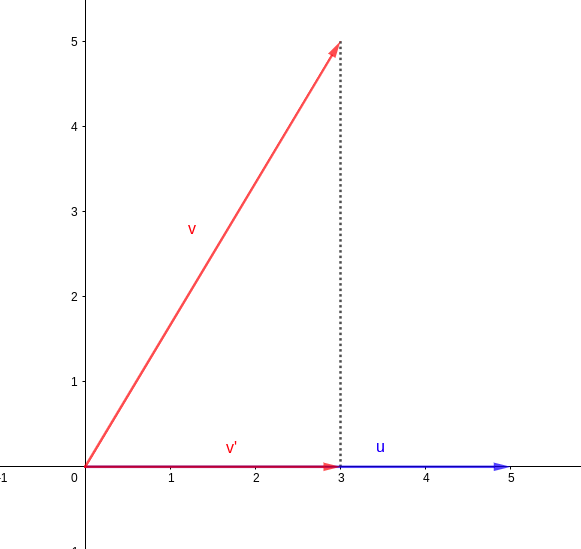
\includegraphics[width=0.5\textwidth]{images/ab.png}
     \caption{Projection of vector $\mathbf{v}$ over $\mathbf{u}$}
    \end{figure}

    
    
    \item Let’s consider $u = (u_i)_{1 \leq i \leq 5}$ and $v = (v_i)_{1 \leq i \leq 5}$, two vectors of length 5.
    How would you clearly write the following part of script using some mathematical notations.
    
    \begin{minted}
    [frame=lines,
    		framesep=2mm,
    		linenos]
    {python}
    # import numpy library as np in order to work on tensors
    import numpy as np
    # create 2 random vectors of length 5
    u = np.random.randn(5)
    v = np.random.randn(5)
    # perform some computations
    r = 0
    for ui, vi in zip(u, v) :
        r += ui * vi
    \end{minted}
    Name the mathematics behind and rewrite the last 3 lines of code in one.
    
    \hrulefill\\
    The last lines of the program perform a scalar product between the two vectors $u$ and $v$ (taking two vectors and returns a scalar) $\mathbf{u}\cdot \mathbf{v}=\displaystyle\sum_{i} u_{i}v_{i}$ The \texttt{zip()} function takes two lists of same size and creates a list of tuples with the values of the two lists. The last line multiply the two values of each tuples and sum all these products (which corresponds indeed to the formula of the scalar product)\\
    We can rewrite those three line as \texttt{r=np.dot(u,v)} (using the numpy library)\\


    \item Complete the code to construct a vector $v$ orthogonal to the vector $u$ and of the same norm.
    Comment each line of your code.
    
    \hrulefill\\
    The code can be found in the file \texttt{ex2.py}

\end{enumerate}

% 
% 
%%%%% ================================================================ %%%%%
\clearpage
\section{Computing Eigenvalues, Eigenvectors, and Determinants}

\begin{enumerate}
    \item Find the determinant, eigenvectors, and eigenvalues of the matrix
    \[
    \begin{bmatrix}
        1 & 1 & 3 \\
        1 & 5 & 1 \\
        3 & 1 & 1
    \end{bmatrix}
    \]
    Compare your results with computer’s one.
    
    \hrulefill \\
    We compute the determinant, the eigenvectors and the eigenvalues of the matrix $A=\begin{bmatrix}
    1 & 1 & 3 \\ 
    1 & 5 & 1 \\ 
    3 & 1 & 1
    \end{bmatrix} $. \\
    \\
    determinant : $det(A)=1\times(5\times1-1\times1)+(-1)\times(1\times1-1\times3)+3\times(1\times1-5\times3) =4+2-42=-36$     \\
    \\
    eigenvalues : $det(A - I\lambda)= 0 <=> det\left( \begin{matrix} (1 - \lambda) & 1 & 3 \\ 1 & (5 - \lambda) & 1 \\ 3 &     1 & (1 - \lambda) \end{matrix} \right) = 0= (1 - \lambda) \times (4 - 6\lambda + \lambda^{2}) - 1 \times (2 + \lambda)     + 3 \times (1 - 15 + 3\lambda) = -36 + 7\lambda^{2} - \lambda^{3} = -(\lambda + 2)(\lambda - 3)(\lambda - 6)$\\
    The eigenvalues are $\{-2, 3, 6\}$\\
    eigenvectors : We solve $(A-\lambda I)\mathbf{v}=\mathbf{0}$ for each possible $\lambda$ to fin the eigenvectors and     we find :\\
    $\mathbf{v}=(-1,0,1)$ for $\lambda =-2$, $\mathbf{v}=(1,-1,1)$ for $\lambda =3$ and $\mathbf{v}=(1,2,1)$ for $\lambda     =6$

    
    \item The covariance matrix for n samples $x_1, \dots, x_n$ , each represented by a $d \times 1$ column vector, is given by
    \[
    C = \frac{1}{n - 1} \sum^n_{i=1} (x_i - \mu)(x_i - \mu)^T,
    \]
    where $C$ is a $d \times d$ matrix and $\mu = \sum^n_{i=1} x_i/n$ is the \textit{sample mean}.
    Prove that $C$ is always positive semidefinite. (Note: A symmetric matrix $C$ of size $d \times d$ is \textit{positive semidefinite} if $v^T C v \geq 0$ for every $d \times 1$ vector $v$.)
    
    \hrulefill \\
    
    
    \item In this portion of the exercise, we will calculate the eigenvalues of the covariance matrices of six data sets listed as follows:
    \begin{table}[H]
    \centering
    \begin{tabularx}{.7\textwidth}{rccX}
    \hline
    filename                          & $n$  & $d$ & description                                                          \\ \hline
    \texttt{tp1\_artificialdata[1-3]} & 1024 & 100 & Artificial data generated from various auto-regression (AR-1) models \\
    \texttt{tp1\_artificialdata4}     & 1024 & 100 & Random Gaussian data                                                 \\
    \texttt{tp1\_freyfaces}           & 1965 & 560 & Facial images of a man named Brendan                                         \\
    \texttt{tp1\_digit2}              & 5958 & 784 & Hand-written images of "2"                                           \\ \hline
    \end{tabularx}
    \end{table}
    To access each data set, go to ''TP1/data'' and download \texttt{tp1\_*}.
    Each file contains a $n \times d$ data matrix with rows representing $n$ different samples in $\mathbb{R}^d$
    For example, \texttt{tp1\_artificialdata1} contains a data matrix of size $1024 \times 100$ (1024 samples, 100 features).
    Once each dataset has been imported into \texttt{Python}, complete the following tasks:
    
    \begin{enumerate}[label=(\alph*)]
        \item Compute the covariance matrix of each dataset;
        
        \item Compute the eigenvalues for each covariance matrix;
        
        \item Compute the determinant of each covariance matrix;
        
        \item Compute the product of the eigenvalues for each covariance matrix;
        
        \item Display the eigenspectrum for each covariance matrix in a 2D plot, where the $x$-axis shows the rank of the eigenvalues, ranging from 1 (the largest eigenvalue) to 100 (the 100-th largest eigenvalue), and the $y$-axis shows the corresponding eigenvalue.
    \end{enumerate}
    Describe the relationship between the product of the eigenvalues and the determinant of each covariance matrix.
    In addition, describe the observations you make regarding the plot of the spectrum of eigenvalues of each covariance matrix.

    \hrulefill \\
    The code can be found in the file \texttt{ex3.py}

\end{enumerate}

%%%%% ================================================================ %%%%%
\clearpage
\section{Computing Projection Onto a Line}
There are given a line $\alpha : 3x - 2y = -6$ and a point $A$ with the coordinates (5, 4).
\begin{enumerate}
    \item Find a distance from the point $A$ to the line $\alpha$
    \item Explain your code using a sketch and some mathematics (there should be a scalar product somewhere).
\end{enumerate}

\hrulefill \\
We want to find the distance between $A(5, 4)$ and the line $\alpha : 3x - 2y = -6$. We start by rewriting $\alpha$ as the function $\alpha (x)=\frac{-6 +2y}{3}$. Then we pick two values $x_{1}$ and $x_{2}$ and compute $\alpha (x_{1}=y_{1})$ and $\alpha (x_{2}=y_{2})$. We compute a vector $\mathbf{u}$ collinear to $\alpha$: $\mathbf{u} = \begin{bmatrix} x_{2} - x_{1}\\y_{2} - y_{1} \end{bmatrix}$. Then we compute $\mathbf{v}$, a vector between a point of $\alpha$ and $A$ : $\mathbf{v} = \begin{bmatrix} x_{1} - A_{x}\\y_{1} - A_{y} \end{bmatrix}$. We compute two vectors, $\mathbf{w_{1}}$ the projection of $\mathbf{v}$ over $\mathbf{u}$ and $\mathbf{w_{2}} = \mathbf{v}-\mathbf{w_{1}}$. Since $\mathbf{w_{2}}$ is collinear to $\mathbf{u}$, $||\mathbf{w_{2}}||$, corresponds to the distance between $A$ and $\alpha$.\\
\\
The code can be found in the file \texttt{ex4.py}


% 
% 
%%%%% ================================================================ %%%%%
% \section*{Submission}
% Please archive your report and codes in "Prénom Nom.zip" (replace "Prénom"
% and "Nom" with your real name), and upload to "Upload Tps > Upload TP1" on
% \url{https://moodle.unige.ch} before \textcolor{red}{Monday, October 10 2022, 23:59 PM}. \\
% Note, the assessment is mainly based on your report, which should include your answers to all questions and the experimental results.
% \textit{Importance is given on the mathematical explanations of your works and your codes should be commented}
% Please use this \href{https://www.overleaf.com/read/fxgrxcvxkmtk}{overleaf template}.

\section*{Supplements}
\begin{enumerate}
    \item Define and explain the mean and the variance on some examples.
    \item Define and explain what is a vector space, a projection and a scalar product.
    \item Define and explain what is a vector space, a basis and a change of basis
transformation matrix.
    \item Present the eigen-value decomposition and the singular-value decomposition.
    \item Be ready to answer questions from slide 37 \textit{DS.02.highDimension}.
\end{enumerate}


%
% %
% % %
% % % %
% % % % %
\end{document}
